\chapter{Анализ проблемы} \label{ch1}

% не рекомендуется использовать отдельную section <<введение>> после лета 2020 года
%\section{Введение. Сложносоставное название первого параграфа первой главы для~демонстрации переноса слов в содержании} \label{ch1:intro}

В данной главе произведён анализ существующих подходов к проблеме  решения. Предложены постановка и формализация задачи целочисленной оптимизации с ограничениями в контексте управления режимом работы светофора.
\section{Анализ существующих решений}
На сегодняшний день уже существуют различные способы решения проблемы расчётов режимов СО. У каждого из способов есть свои преимущества и недостатки. Естественно заметить, что длительности действия сигналов светофоров должны устанавливаться в соответствии имеющимся на дорожном участке потоком машин.\\
Например, в \cite{fuzzy-logic} предлагается алгоритм на основе машинного обучения с подкреплением и нечеткой логики. Подход применяется к каждому отдельно взятому СО, обрабатывающему входящий поток машин (учитывается расстояние от каждого отдельного ТС до перекрестка) при помощи вышеупомянутых алгоритмов.\\
В статье \cite{dynamic-programming} описано использование динамического программирования для каждого отдельно взятого светофора. Недостатком модели, представленной в этой статье является неточная модель трафика: используются только данные о количестве ТС пересёкших перекресток, регулируемый СО, в течение времени действия фазы.\\
Ещё одним вариантом решения проблемы является \cite{machine-learning}. Выполняется микромоделирование дорожного участка и генерируется автомобильный трафик. К сожалению, с увеличением дорожной сети длительность подсчёта ЦФ кратно увеличивается, поэтому для снижения времени подсчёта ЦФ используются суррогатных моделей на основе нейросети или моделей, построенных при помощи градиентного бустинга. Оптимизация длительностей фаз производится при помощи алгоритмов оптимизации, таких как генетический алгоритм, метод имитации отжига и др. Недостатком такого решения является тот факт, что дорожный трафик не является моделью, построенной на реальных данных.\\
Подход, описанный в \cite{Sun2006BilevelPF}, представляет проблему расчётов режимов СО как двухуровневую задачу оптимизации. Задачей верхнего уровня является расстановка длительностей действия сигналов, а задачей нижнего уровня - распределение дорожного трафика. Недостатком этой работы является вычислительная сложность и факт, что трафик построен не на реальных данных, а приближен моделью Reactive Dynamic User Assignment (RDSUO).\\
Примером подходов с весьма значительными допущениями, такими как:
\begin{itemize}
	\item Прохождение только одной машины через перекресток в текущий момент времени.
	\item Ограничение на количество сигналов: только красный и зелёный.
	\item Ограничение на количество дорожных полос.
	\item Обязательное равенство времени действия красного и зелёного сигналов.
	\item Ограничение на количество фаз: две.
	\item Обязательное равенство длительностей фаз.
\end{itemize}
являются статьи \cite{Chen2007AlgorithmsFT} и \cite{PSO-weak}.\\
В данной работе предлагается избавиться от недостатков подходов к решению проблемы, описанных выше, следующим образом:
\begin{itemize}
		\item Построить точную микромодель. Поток ТС смоделировать на основании реальных данных, полученных с дорожных радиодетекторов. Расстановки сигналов СО, времена длительностей фаз построить по паспортам СО. Данные о дорожной разметке на исследуемом участке взять из открытых источников (Google Maps, Яндекс Карты).
		\item Не использовать суррогатные модели, чтобы не терять в точности полученного решения. Для приемлемого времени работы алгоритмов не использовать модели больших дорожных участков.
		\item Снять ограничения на длительности фаз, количество и цвет сигналов.
		\item Использования наиболее эффективной модели движения автомобильного трафика "разумного водителя" $ $ (Intelligent Driver Model, IDM).
\end{itemize}
\newpage
\section{Задание дорожной сети}
Участок транспортной сети опишем в виде ориентированного графа $\Gamma(V,E)$, где $V$ - множество вершин, $E$ - множество дуг сети.\\
Из $V$ выделим подможества $S\subseteq V$, $D\subseteq V$ и дадим определения:
\begin{itemize}
	\item \textit{Источником} называется элемент множества $S$, который порождает транспортный поток.
	\item \textit{Стоком} называется элемент множества $D$, который поглощает транспортный поток.
\end{itemize}

Каждая дуга соответствует реальному участку автодороги без перекрёстков\\
(дорожной полосе). Каждая вершина представляет собой либо перекрёсток, регулируемый светофорным объектом, либо является источником, либо стоком либо источником и стоком одновременно.
\begin{m-definition} \cite{book-Gasnikov}
	Множество $W$ всех потокообразующих пар представим в виде декартова произведения 
	\begin{equation}
		W = S \times D = \{\omega = (i, j): \ i \in S, j \in D\}
	\end{equation}
\end{m-definition}
\begin{m-definition} \cite{book-Gasnikov}
	Путём (маршрутом) в сети $\Gamma$, соединяющим вершины $i$ и $j$, назовём последовательность дуг
	\begin{equation}
		e_1 = (i\rightarrow k_1), \ e_2 = (k_1 \rightarrow k_2), \ \ldots, \ e_m = (k_{m-1} \rightarrow k_m), \  e_{m+1} = (k_m \rightarrow j)
	\end{equation}
	где $e_l \in E$ при всех $l = 1,\ldots, m+1$
	
\end{m-definition}
В маршрутах предполагается отсутствие петель и циклов.
Обозначим через $P_w$ \cite{book-Gasnikov} множество альтернативных маршрутов, связывающих пару $w \in W$.
Совокупность всех путей в сети $\Gamma$ обозначим через $P = \underset{\omega \in W}{\cup}P_{\omega}$.
Пользователями дорожной сети будем считать только автомобили.
Автомобили перемещаются по маршрутам из $P$.

\section{Задание светофорного цикла}
\begin{m-definition}\cite{book-Novikov}
	Пусть $\Gamma(V, E)$ - граф. Пусть $v_1, v_2 \in V$ вершины, $e = (v_1, v_2) \in E$ - соединяющее их ребро. Говорят, что $v_1$ \textit{инцидентна} ребру $e$, а также $e$ \textit{инцидентно} вершине $v_2$.
\end{m-definition}
Выделим из множества $V$ подмножество $O \subset V$, $|O| = N, N \in \mathbb{N}$ вершин - светофорных объектов. $o_i\in O, \ i \in 1,\ldots, N$ регулируют состояние потока автомобилей на инцидентных $o_i$ дугах, входящих в $o_i$, с помощью сигналов.
\begin{m-definition}
		Сигнал светофорного объекта - визуальный сигнал, регулирующий движение ТС в дорожной сети.
\end{m-definition}
Введём три вида сигналов:
\begin{itemize}
	\item \textit{Красный} - предупреждает о том, что движение потока ТС должно быть приостановлено в течение времени активности сигнала.
	\item \textit{Желтый} - информирует о предстоящей смене красного сигнала на зелёный.
	\item \textit{Зелёный} - разрешает дальнейшее движение ТС по дорожной сети.
\end{itemize}

Объединим сигналы в множество $\mathcal{L} = \{ l_i \}, \ i = 1, \ldots, M, \ M \in \mathbb{N}.$\\
Для уточнения, каким образом сигналы управляют потоком на инцидентных входящих дугах, введём определение фазы.
\begin{m-definition}
	Фаза - это пара, содержащая \textit{состояние} $l$-го светофорного объекта, поддерживаемое СО в течение времени действия фазы $t_{lk}$, и само время действия фазы $t_{lk}$, где $k$ - номер фазы $k \in 0, \ldots, K$. 
\end{m-definition}
Допустимо различное количество фаз для различных светофоров.
\begin{m-definition}
	Под \textit{состоянием} понимается совокупность влияний сигнала $l_i$ на дуги $e_j, \  j \in \{1,\ldots, N\}$ в фазе $t_{lk}$, $t_{\min} \leq t_{lk} \leq t_{\max}$, \ $[t_{lk}] = \text{с}$.\\
\end{m-definition}
Предлагается применить алгоритмы оптимизации к временам действия фаз $t_{lk}$.\\

\begin{figure}[!htbp]
	\adjustbox{minipage=1.3em,valign=t}{\subcaption{}\label{fig:state-a}}%
	\begin{subfigure}[t]{\dimexpr.3\linewidth-1.3em\relax}
		\centering
		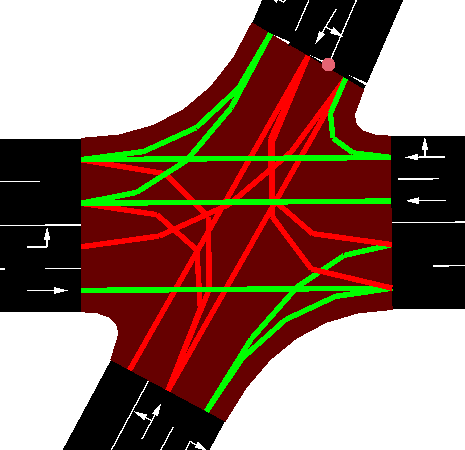
\includegraphics[width=.60\linewidth,valign=t]{my_folder/images//separate-state-0.png}
	\end{subfigure}
	\hfill %выровнять
	\adjustbox{minipage=1.3em,valign=t}{\subcaption{}\label{fig:state-b}}%
	\begin{subfigure}[t]{\dimexpr.3\linewidth-1.3em\relax}
		\centering
		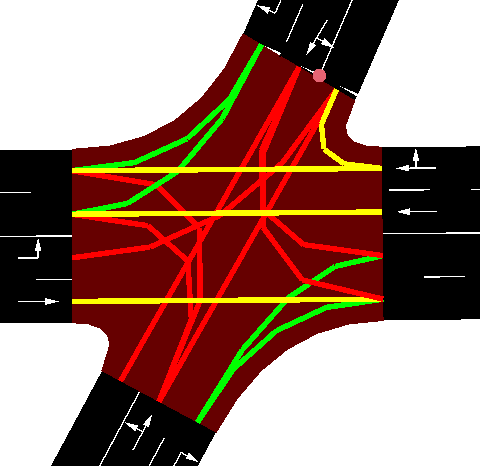
\includegraphics[width=.60\linewidth,valign=t]{my_folder/images//separate-state-1.png}
	\end{subfigure}
	\hfill %выровнять
		\adjustbox{minipage=1.3em,valign=t}{\subcaption{}\label{fig:state-c}}%
	\begin{subfigure}[t]{\dimexpr.3\linewidth-1.3em\relax}
		\centering
		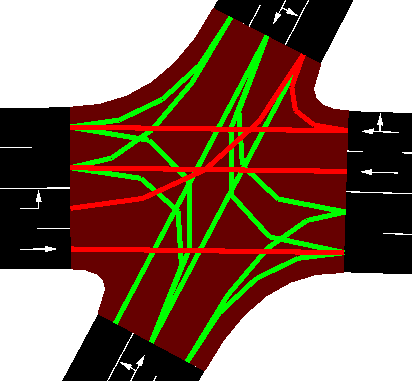
\includegraphics[width=.60\linewidth,valign=t]{my_folder/images//separate-state-2.png}
	\end{subfigure}%
\captionsetup{justification=centering} %центрировать
\caption{Пример смены состояний {\itshape a} $\rightarrow$ {\itshape b} $\rightarrow$ {\itshape c}}
\end{figure}




 
\section{Постановка задачи оптимизации}
Пусть $X = \biggr[t_{lk}\biggl]_{\begin{aligned}
		\scriptstyle l & \scriptstyle \in 1,\ldots, N,\\
		\scriptstyle k & \scriptstyle \in 0, \ldots, K
\end{aligned}}, X \in \mathbb{R}^{N\times K}$ вектор, содержащий длительности фаз светофорных объектов.\\
Введём:
\begin{itemize}
	\item $T$ - продолжительность времени симуляции трафика.
	\item $N$ - количество ТС, преодолевших полные намеченные пути (маршруты) за время $T$.
\end{itemize}
\begin{m-definition}
	\textit{Временем ожидания} (\textit{простоя}) $\tau_i(X)$ $i$-ого ТС назовём время, в течение которого скорость $v$ ТС удовлетворяет ограничению $v < 0.1 \ \frac{\text{м}}{\text{c}}$.\\
\end{m-definition}
Пусть $\tau_i$ - время ожидания $i$-ой машины. Тогда
\begin{equation}
	\displaystyle f(X) = \frac{\sum\limits_{i = 1}^{N}\tau_i}{N}
\end{equation} - функция цели.
Тогда в финальном виде задача оптимизации будет выглядеть следующим образом:
\begin{equation}
	\label{eq:goal-function}
	\begin{aligned}
		\min_{X} \quad & f(X) \\
		\text{s.t.} \quad & t_{lk} \in [t_{\min}, t_{\max}]\
	\end{aligned}	
\end{equation}

%\FloatBarrier % заставить рисунки и другие подвижные (float) элементы остановиться

%% Вспомогательные команды - Additional commands
%
%\newpage % принудительное начало с новой страницы, использовать только в конце раздела
%\clearpage % осуществляется пакетом <<placeins>> в пределах секций
%\newpage\leavevmode\thispagestyle{empty}\newpage % 100 % начало новой страницы